%%%%%%%%%%%%%%%%%%%%%%%%%%%%%%%%%%%%%%%%%%%%%%%%%%%%%%%%%%%%%%%%%%%%%%%%%%%%%%%%
\section{Evaluation}
\label{sec:eval}

\subsection{NaN Analysis}
\label{sec:nan}

In this section, we provide an analysis of the probability that the LLM outputs NaN. \\

Let $F$ be an LLM model with $n$ parameters and $x$ be the input to the model. We would like to find $Pr(F(x) = NaN)$.

Suppose a bit is flipped with probability $p$.

Let $X$ be the value of a model parameter and $X^*$ be its perturbed value. Note that parameters are iid $\sim Uniform(0, 1)$ due to the design of LLMs [do you have a good source for this allen]. According to \cite{IEEE754}, a NaN value has all 1s in the exponent field, and a nonzero mantissa. Since $0 \le X \le 1$, the exponent field is $01111111$ (due to the +127 offset), and suppose there are $j$ 1s in the mantissa. \\

Then, $X^* = NaN$ if the remaining exponent bit flipped, the rest of the exponent bits don't flip, and not all $j$ mantissa bits turn to 0. Thus,
\begin{align*}
	Pr(X^* = NaN) &= Pr(\text{only one exponent bit is flipped}) \\
    & \quad \cdot (1 - Pr(\text{all mantissa bits are 0})) \\
	&= p(1 - p)^7 * (1 - p^j(1 - p)^{23 - j})
\end{align*}

We can represent the value of mantissa as a random variable $\sim Binom(23, 0.5)$. Thus,

\begin{align*}
	Pr(X^* = NaN) &= \sum_j^{23} Pr(X^* = NaN \mid X \text{ has $j$ mantissa 1s}) \\
    & \quad \cdot Pr(X\text{ has $j$ mantissa 1s}) \\
	&= \sum_j^{23} p(1 - p)^7 * (1 - p^j(1 - p)^{23 - j})\binom{23}{j}0.5^j0.5^{23 - j} \\
	&= 2^{-23} p (1 - p)^7 \left(\sum_{j=0}^{23}[1 - p^j(1 - p)^{23 - j}] \binom{23}{j}\right) \\
	&= 2^{-23} p (1 - p)^7 \left(\sum_{j=0}^{23}\binom{23}{j} - \sum_{j=0}^{23}p^j(1 - p)^{23 - j} \binom{23}{j}\right) \\
	&= 2^{-23} p (1 - p)^7(2^{23} - 1) \\
	&= p(1 - p)^7(1 - 2^{-23})
\end{align*}

Now putting everything together, we note that the model will output NaN if any of the parameters of the model are NaN, due to NaN propagation. Thus,

\begin{align*}
	Pr(F(x) = NaN) &= Pr(\text{at least one parameter is NaN}) \\
	&= 1 - Pr(\text{all parameters are not NaN}) \\
	&= 1 - \prod_{i=1}^n Pr(X_i \neq NaN) \\
	&= 1 - Pr(X^* \neq NaN)^n \\
	&= 1 - (1 - Pr(X^* = NaN))^n \\
	&= 1 - (1 - p(1 - p)^7(1 - 2^{-23}))^n
\end{align*}

For $p = 10^{-9}$ and $n \approx 130 * 10^6$ (GPT-2), we get $Pr(F(x) = NaN) \approx 0.1$, and for $p = 10^{-8}$, we get $Pr(F(x) = NaN) \approx 0.7$, which explains why at a low error rate, the model still outputs NaN quite consistently.

\subsection{Variation by Layer}

\subsubsection{Probability Variation}
We began by analyzing, at each level, how variations in probability effect the evaluation on the MMLU benchmark at various probability from $1e-7$ to $1e-3$.

As mentioned before, for computational reasons we grouped up layers into groups of size $4$. For ease of viewing this result, we only present the value for layer groups $1, 2, 7$ and $8$. A similar pattern
holds for all unshown groups.

Below are our results for each layer group with various probabilities.

\begin{figure}[!htbp]
    \centering
    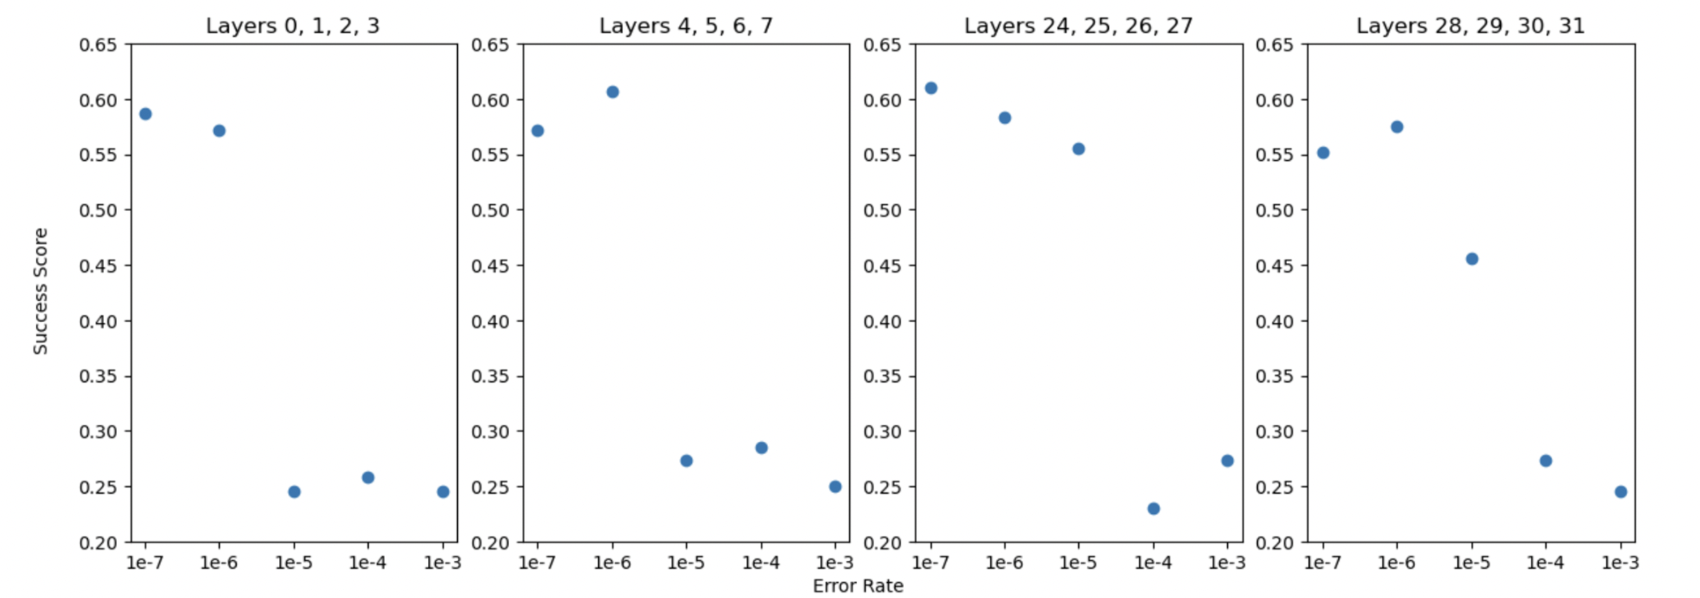
\includegraphics[width=1.0\textwidth]{images/varyprob.png}
    \caption{Score when Varying Probability}
    \label{fig:varyprob}
\end{figure}

As one can notice, for probabilities $1e-6$ (this is about 200 total errors for each layer group) there is no noticeable negative effect that our injected errors have on the model.

On the other hand, for probabilities $1e-4$ (about 20000 total errors), the output of our LLM for each layer that we have is essentially no better than random guessing, no matter which layer we have injected into.

The only layer where something interesting seems to be happening is at the $1e-5$ parameter, so we look into this further in the below section.

\subsubsection{Zooming in on 1e-5}

\begin{figure}[!htbp]
    \centering
    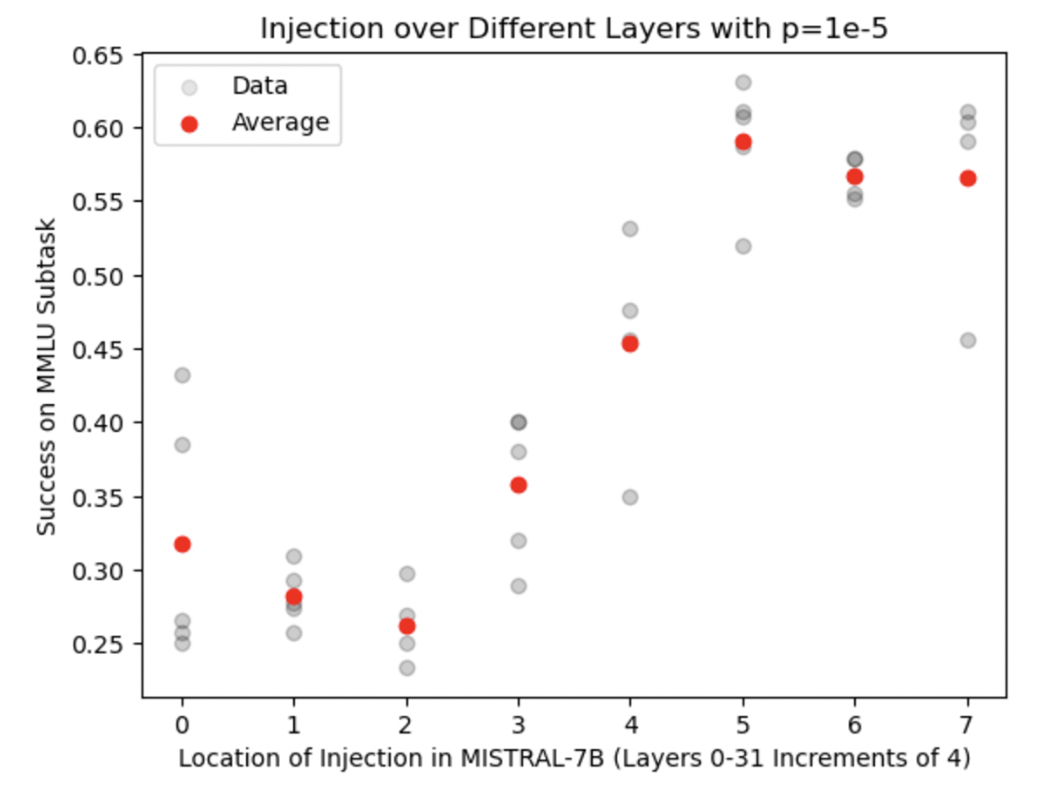
\includegraphics[width=1.0\linewidth]{images/varylayer.png}
    \caption{Score when Varying Layers with p = 1e-5}
    \label{fig:varylayer}
\end{figure}

There are a few interesting things to notice here.

The first is that there does seem to be an effect of the layer on the error injection. For example, errors later layers seem to have less of a degratory effect on the efficacy of the LLM compared to earlier layers.
This is certainly an interesting result that seems to suggest that errors in earlier layers propagate to later layers.

Another interesting thing to note is that many there does seem to be a large amount of variation. We will explore this in a later section, but for now it suffices to say that this is because the variation in our error injection process
means that some more vulnerable components within the individual layers also have a large effect on the total degradation of the LLM.

\subsection{Variation by Component}
\subsubsection{Probability Variation}
We begin by analyzing, for each LLM component (i.e Attention Mechanism, Embedding, etc) how variations in the likelihood of SDC, from $10^{-9}$ to $10^{-1}$ effect the model's accuracy. Below are these results.

\begin{figure}[!htbp]
    \centering
    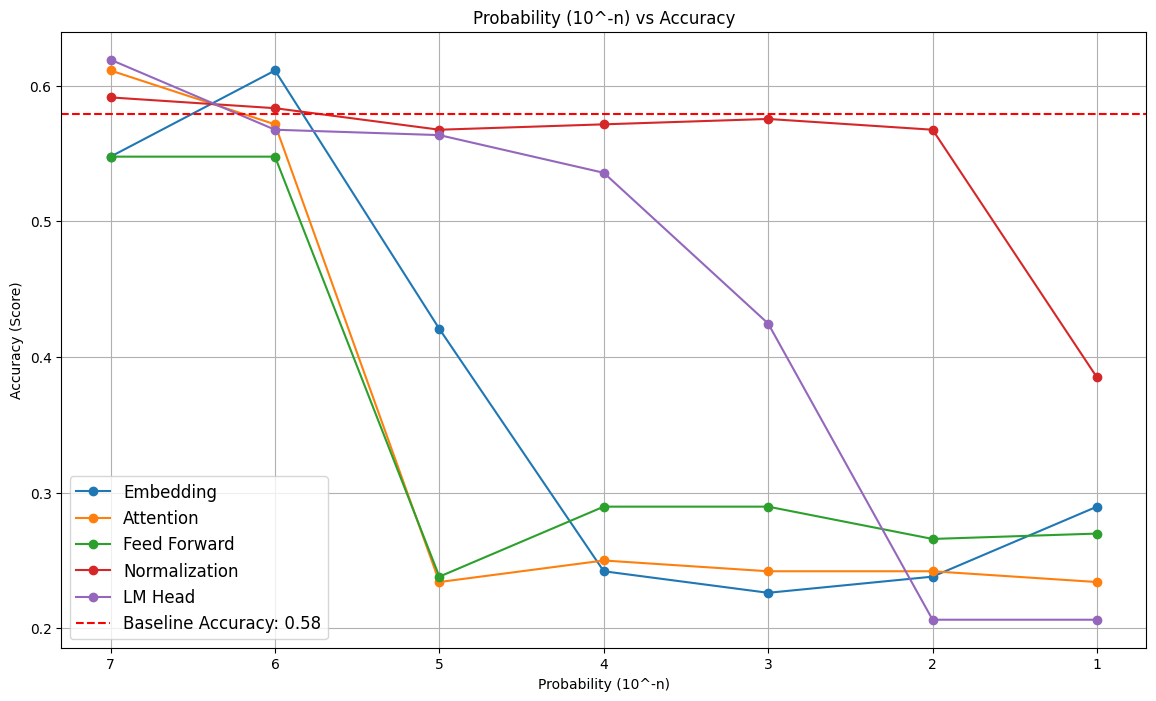
\includegraphics[width=1\linewidth]{images/component-accuracy.png}
    \caption{Likelihood of SDC vs Model Accuracy}
    \label{fig:varcomp}
\end{figure}

From the above results, it is evident that certain components are more sensitive to SDC in terms of model accuracy and performance. To quantify this sensitivity, we calculate the \textbf{Relative Change in Accuracy}. \[
\text{Relative Change in Accuracy} = \frac{\text{Accuracy}_{\text{baseline}} - \text{Accuracy}_{\text{faulty}}}{\text{Accuracy}_{\text{baseline}}}
\]
Below is a graph of this metric for every likelihood.

\begin{figure}[!htbp]
    \centering
    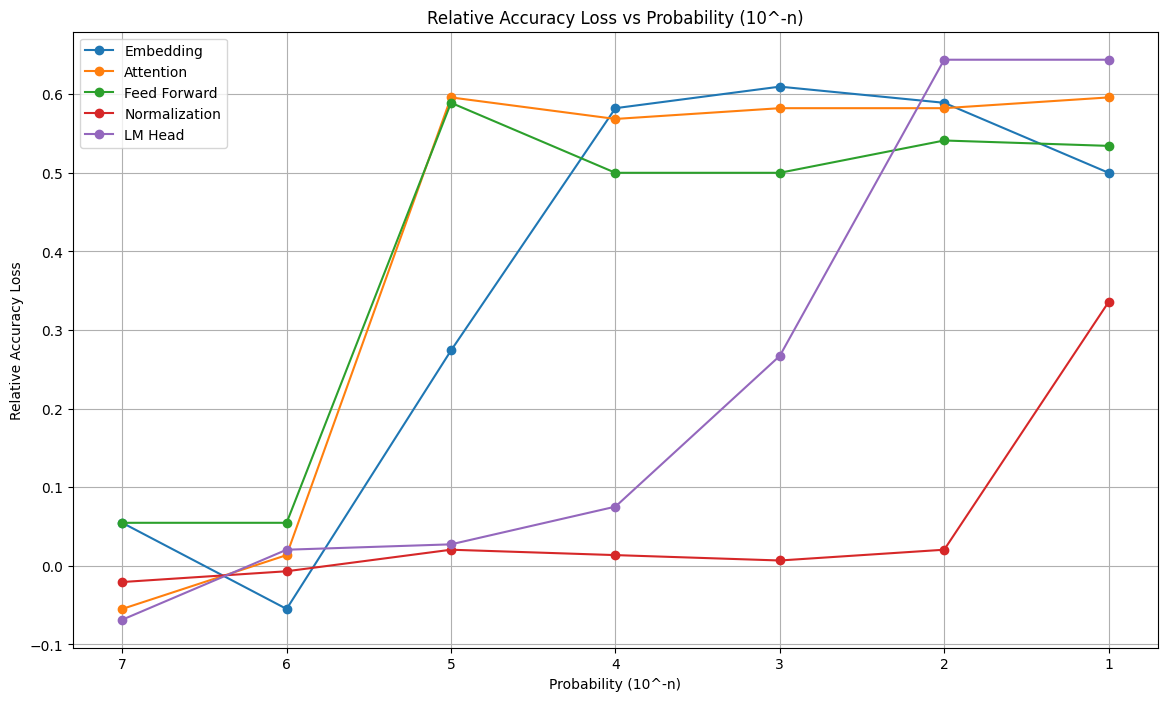
\includegraphics[width=1\linewidth]{images/rel_acc_loss.png}
    \caption{Likelihood of SDC vs Relative Change in Accuracy Loss}
    \label{fig:enter-label}
\end{figure}

This visualization shows us how each component, at each likelihood of SDC, degrades in performance relative to the baseline accuracy of the model. Evidently, components like Normalization and LM Head are much more resilient to SDC than the Feed-Forward and Attention components within the decoder layers of the model.

Furthermore, the thresholds at which model performance degrades by 50\% across components are visualized below:
\begin{figure}[!htbp]
    \centering
    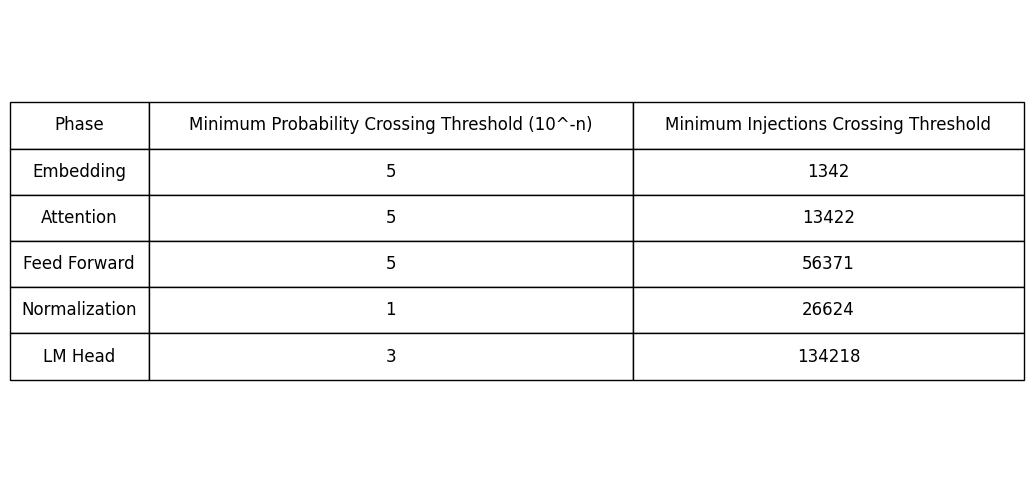
\includegraphics[width=1\linewidth]{images/threshold.png}
    \caption{Thresholds for Model Performance to Degrade Model Performance by 50\%}
    \label{fig:enter-label}
\end{figure}

To develop a comprehensive sensitivity metric for each component, considering all SDC likelihoods, we compute the \textbf{Average Weighted Relative Change in Accuracy Loss (AWRCL)}. \[
\text{AWRCL} = \frac{\sum_{i=1}^{n} w_i \cdot \left( \frac{\text{Accuracy}_{\text{baseline}} - \text{Accuracy}_{i}}{\text{Accuracy}_{\text{baseline}}} \right)}{\sum_{i=1}^{n} w_i}
\]
The ranking of LLM components by this metric is displayed below.

\begin{figure}[!htbp]
    \centering
    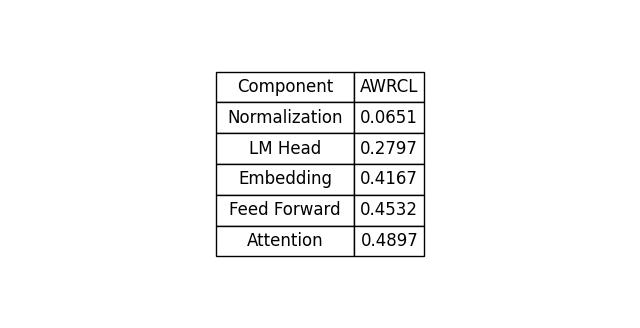
\includegraphics[width=1\linewidth]{images/comp-ranking.png}
    \caption{Ranking of Components by Average Weighted Relative Change in Accuracy Loss with Respect to SDC Likelihood}
    \label{fig:enter-label}
\end{figure}
These results reveal that \textbf{Normalization} and \textbf{LM Head} components are the most resilient to SDC. Notably, the LM Head, responsible for mapping vector representations to vocabulary probabilities, shows remarkable resistance despite its outputs being terminal. This aligns with the general observation that errors in earlier layers have a more pronounced impact on model accuracy. The unexpected resilience of the Normalization component, however, warrants further investigation.

\subsubsection{Normalizing for Component Size}

While the previous analysis compares accuracy degradation by SDC likelihood, components with fewer parameters naturally experience fewer total corruptions. To address this, we normalize the results by the number of parameters in each component, as shown below.

\begin{figure}[!htbp]
    \centering
    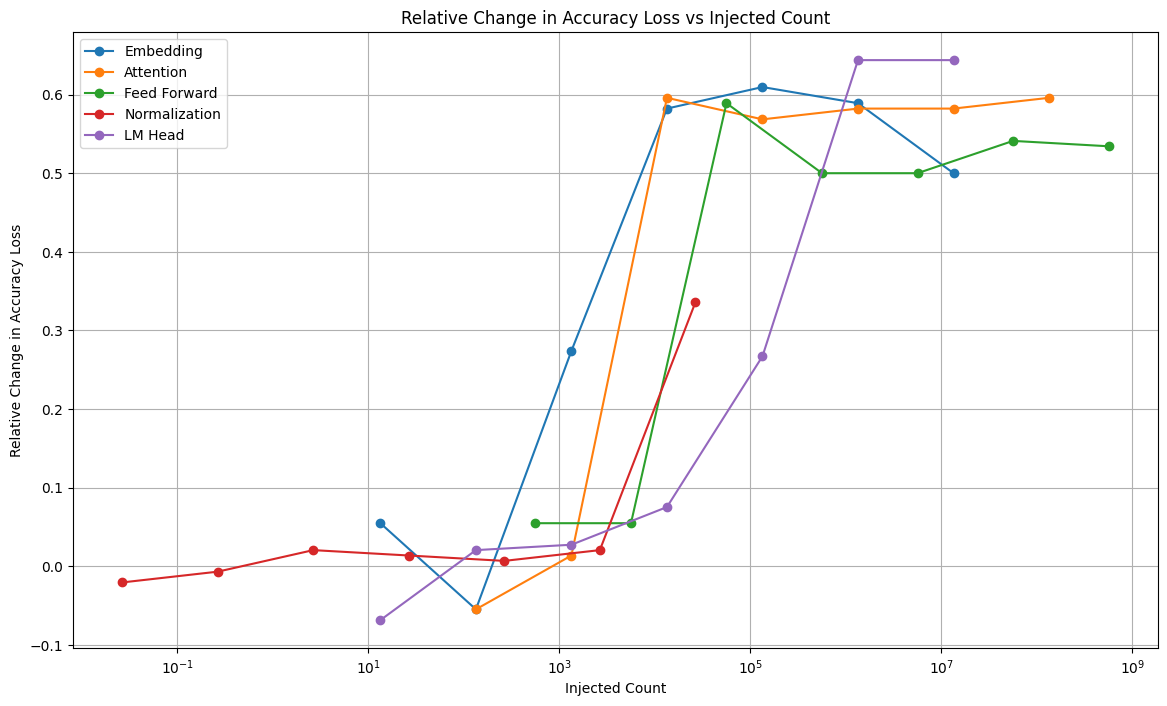
\includegraphics[width=1\linewidth]{images/norm-rel-acc-loss.png}
    \caption{Number of Injected Errors vs Relative Change in Accuracy Loss}
    \label{fig:enter-label}
\end{figure}
The normalized rankings of components, accounting for the number of injected errors, are presented here:

\begin{figure}[!htbp]
    \centering
    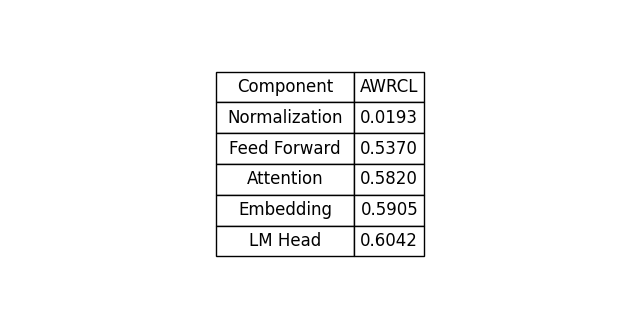
\includegraphics[width=1\linewidth]{images/norm-comp-ranking.png}
    \caption{Ranking of Components by Average Weighted Relative Change in Accuracy Loss with Respect to Injected Error Count}
    \label{fig:enter-label}
\end{figure}

The results suggest that, excluding the Normalization component's AWRCL, the sensitivity of components to SDC becomes roughly similar when normalized for parameter count. This finding highlights that smaller components require a proportionally larger fraction of errors to experience equivalent accuracy degradation compared to larger components. Consequently, smaller components inherently exhibit greater resilience to SDC.

In real-world scenarios, assuming uniform bit error rates across memory, the proportion of errors across components is expected to be similar. Thus, these findings offer practical insights into resource-constrained environments, where prioritizing protection (e.g., using ECC or activation clipping) for specific components is critical.

\subsubsection{Formula to Model Accuracy Degradation}

Through our results, and analysis, we aim to provide a formula to model how sensitive a component is to accuracy degradation as a result of SDC, by identifying key factors.


\[
D \propto N \cdot S_c\cdot P_f \cdot A \cdot (1 - R)
\]

\text{Where:}
\begin{align*}
D & : \text{Performance degradation,} \\
N & : \text{Number of parameters or operations in the component,} \\
S_c & : \text{Sensitivity factor for the component, measured by the AWRCL} \\
P_f & : \text{Fault likelihood (probability of a fault per parameter or operation),} \\
A & : \text{Amplification factor,} \\
R & : \text{Redundancy factor,} \\
\end{align*}

This formula captures the relationships derived from our experiments with sequential layer injections and component-level injections. Notably, the \textbf{Amplification Factor} $A$ encapsulates the tendency for earlier layers to propagate faults more significantly through the model. Conversely, the \textbf{Redundancy Factor} $R$ represents the degree of overlap in calculations, typically higher in larger components.

In the case of the sparse Mistral 7B model, reduced redundancy contributes to greater sensitivity in larger layers, providing additional context to our earlier observation that larger components are generally less resilient to SDC.

